\chapter{\IfLanguageName{dutch}{Stand van zaken}{State of the art}}
\label{ch:stand-van-zaken}

% Tip: Begin elk hoofdstuk met een paragraaf inleiding die beschrijft hoe
% dit hoofdstuk past binnen het geheel van de bachelorproef. Geef in het
% bijzonder aan wat de link is met het vorige en volgende hoofdstuk.

% Pas na deze inleidende paragraaf komt de eerste sectiehoofding.

De literatuurstudie geeft een beeld van de stand van zaken op het vlak van indoor navigatie, vaak afgekort to IN. Er wordt eerst aangehaald welke mogelijkheden er bestaan voor IN en welke problemen er worden tegengekomen wanneer dit in de praktijk wordt gebracht. Daarna volgt er een beschrijving van de verschillende technologieën waarvan een indoor navigatie app gebruik maakt en hoe deze functioneren. Op het einde worden er ook enkele betalende applicaties besproken en wat deze hun capaciteiten zijn.

De bedoeling van deze literatuurstudie is om ontwikkelaars die een nieuwe IN applicatie willen ontwerpen en startpunt te geven van beschikbare technologieën en onderzoek in deze velden. 

\section{\IfLanguageName{dutch}{IDE en Source Code Editor}{IDE and Source Code Editor}}
\label{sec:IDE-codeEditor}

De termen IDE en source code editor, meestal verkort tot code editor, worden vaak door elkaar gebruikt. Er is daarentegen een functioneel verschil tussen deze twee termen. Het verschil wordt verduidelijkt met de volgende definitie:

\begin{displayquote}
"An integrated development environment (IDE) is software for building applications that combines common developer tools into a single graphical user interface (GUI). An IDE typically consists of a Source code editor,  Local build automation and Debugger." \autocite{RedHat2018}
\end{displayquote}

De code editor maakt dus integraal deel uit van de IDE. Deze laatste bevat daarnaast namelijk andere tools zoals een geïntegreerde compiler/interpreter, build-automatisatie, een debugger, versiecontrole, een test framework en soms nog andere tools. Voorbeelden van IDEs in dit onderzoek zijn Visual Studio, Eclipse en IntelliJ.

Onder code editor wordt verstaan dat dit een grafische tekst editor is met extra functionaliteit zoals syntax markering, indentatie, auto-voltooiing en bracket matching. Hieruit kan ook afgeleid worden dat code editors lagere hardware vereisten hebben doordat deze minder functionaliteit hebben. Moderne code editors maken vaak gebruik van plug-ins of extensions om meer functionaliteiten van de IDE aan te bieden. Maar in het algemeen bieden ze dit niet standaard aan en moet de gebruiker dit zelf configureren.

\begin{figure}[h!]
    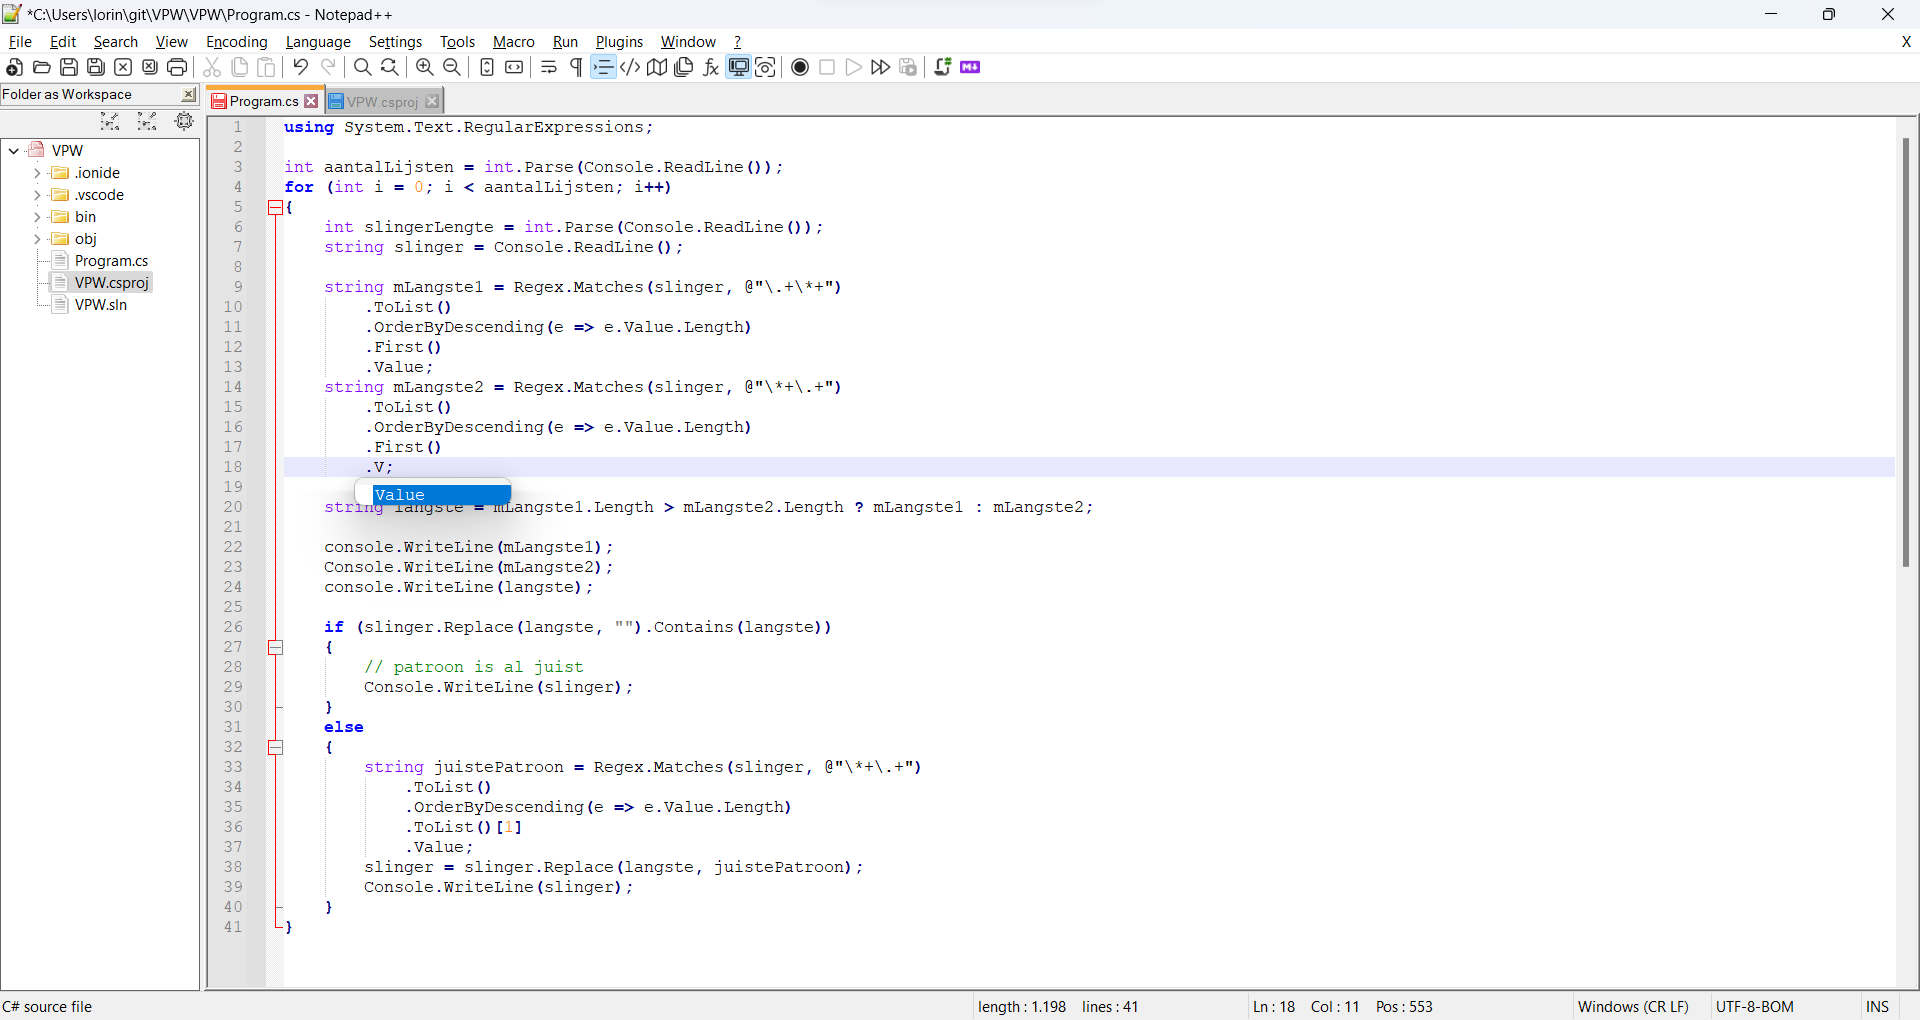
\includegraphics[width=\linewidth]{CodeEditor.png}
    \caption{De Notepad++ code editor}
    \label{fig:codeEditor}
\end{figure}

\begin{figure}[h!]
    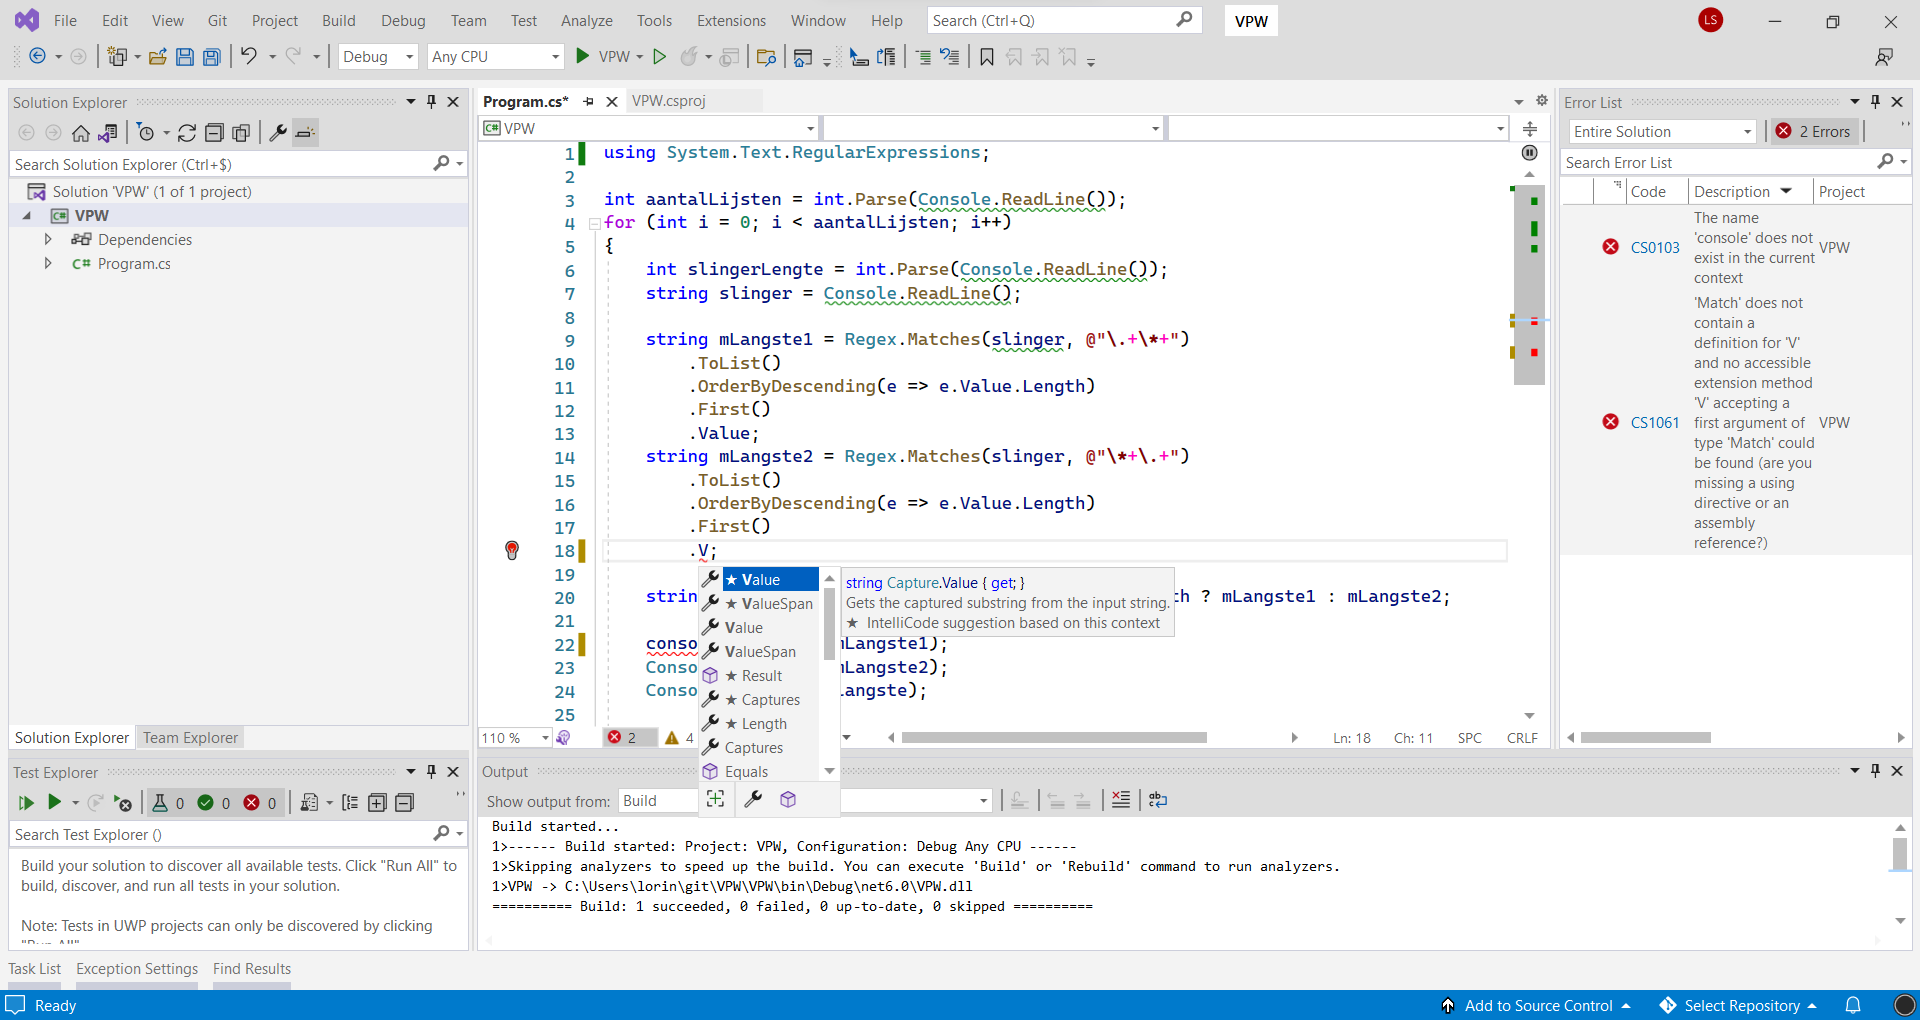
\includegraphics[width=\linewidth]{IDE.png}
    \caption{De Visual Studio IDE}
    \label{fig:IDE}
\end{figure}

Als illustratie zijn 2 afbeeldingen van hetzelfde project gegeven om het verschil in functionaliteit tussen de code editor en de IDE te verduidelijken. Op het eerste gezicht zijn deze vrij gelijkend, een tekst editor die centraal staat met daarrond wat vensters en knoppen. Maar bij nader inzicht is het duidelijk dat de IDE meer aanbiedt, zoals sterkere syntax markering(meer sleutelwoorden worden gekleurd), context bewuste aanvulling (het menu onderaan de V), error controle(lijst van errors en rood onderlijnde code), build en run uitvoer, testen, debugging via breakpoints...

\section{\IfLanguageName{dutch}{Ontstaan van de IDE}{Origin of the IDE}}
\label{sec:IDE-ontstaan}

De eerste IDE is ontwikkeld in 1980, nadat programmeertalen overschakelden naar ontwikkeling via de console. Dit was hiervoor niet mogelijk omdat de eerste software geprogrammeerd werd met ponskaarten. De eerste computertaal die bewerkt kon worden met een IDE was Dartmout basic. Deze IDE was gelimiteerd in functionaliteit en werd niet bestuurd met een GUI, maar met console commando's. Het doel van deze eerste IDE, net zoals nu, was om de productiviteit van de programmeur te verhogen \autocite{JAXenter2018}.

Dit gebeurde door de verschillende tools die een programmeur nodig had om software te maken, te combineren. Dit zorgde voor een reductie in ontwikkelingstijd omdat in de oude workflow veel manuele taken zaten. Eerst werd het programma opgesteld in een standaard tekst editor. Daarna werd het bestand met de geschreven code door de compiler vertaald en werden de errors die deze teruggaf manueel op papier overgezet. Daarna werd de cyclus voltooid door terug naar de tekst editor te gaan om deze errors op te lossen. Dit was natuurlijk een zeer inefficiënte workflow.

De eerste IDEs hadden wel problemen, ze waren bijvoorbeeld moeilijk in gebruik en hadden een grote leercurve, soms was zelfs professionele training nodig. Dit zorgde ervoor dat ze niet tot hun volledige potentieel gebruikt werden, of zelfs helemaal niet. Uit onderzoek van \textcite{Kline2005} werd er opgemerkt dat 70\% van CASE tools (computer-assisted software engineering tools, waaronder IDEs vallen) een jaar na aankoop niet meer gebruikt werden. Hier kwam dan ook bij dat de aanschaffingskosten heel hoog waren, deze konden oplopen tot \$20,000 per ontwikkelaar.

Samen met de steeds groeiende hardware mogelijkheden en de verspreiding van Windows kwamen de GUI gebaseerde IDEs op. Deze werd gepionierd door Visual Basic, de eerste in de markt met drag en drop functionaliteit \autocite{Kiong2019}. De volgende IDE die de markt voortstuwde was Visual Studio met zijn eerste uitgave in 1997. Dit was een van de eerste IDEs die niet enkel bedoeld was om voor 1 specifieke computertaal te werken, maar voor verschillende tegelijk.

\section{\IfLanguageName{dutch}{Nood van IDEs in de moderne ontwikkelingsomgeving}{Need of IDEs in the modern developement environement}}
\label{sec:IDE-nood}

Nu na jarenlange ontwikkeling is de IDE een belangrijke tool in het arsenaal van programmeurs, en zijn er vele verschillende opties voor elke taal en framework. Als er naar volgend onderzoek van \textcite{Tidelift2019} gekeken wordt, kan er opgemerkt worden dat het merendeel van de tijd van de ontwikkelaar in de IDE wordt doorgebracht. Hierbij zijn de bevindingen dat er 32\% effectief besteed wordt aan het schrijven van nieuwe code, wat in de IDE uitgevoerd wordt. Daarnaast wordt er 19\% van de tijd aan code management en 12\% aan testen besteed, wat mogelijk is gemaakt door de geïntegreerde refactoring en test tools van IDEs. Samen betekende dit dat 63\% van de tijd van de ontwikkelaars in de IDE wordt doorgebracht, hieruit volgt dus de nood voor performante IDEs.

\section{\IfLanguageName{dutch}{Prominente IDEs}{Prominent IDEs}}
\label{sec:IDE-prominent}

Er is momenteel een groot aanbod van IDEs verkrijgbaar, sommige betalend en sommige gratis. De meeste IDEs focussen zich op lichtelijk andere doeleinden, sommigen leggen zich toe op 1 specifieke programmeertaal of framework en bieden hier dan diepgaande integraties voor aan. Er zijn ook andere IDEs die minder specifiek gaan en waarbij de gebruiker zelf de verschillende programmeertalen moet configureren, dit is dan meestal in de vorm van extensions. De verschillende IDEs hebben ook verschillende groottes van gebruikersgroepen, de ene is al populairder als de andere. Deze studie zal zich bezighouden met enkele van de meest populaire IDEs, zoals gevonden in de \textcite{StackOverflow2021} Developer Survey. De IDEs opgenomen in dit onderzoek zijn Visual Studio Code, Visual Studio, Eclipse, IntelliJ, en Notepad++.

\subsection{Visual Studio Code}
%- Github repo
%- Monaco editor and electron
%https://stackoverflow.com/questions/29966093/what-is-the-visual-studio-code-editor-built-on
%https://code.visualstudio.com/docs/editor/whyvscode

Visual Studio Code\footnote{https://code.visualstudio.com/}, afgekort tot VS Code, is een open source code editor ontwikkeld door Microsoft. Deze editor is volledig gratis en heeft geen betalende opties. VS Code is een van de jongere editors, met zijn originele uitgave in 2015. VS Code is ook populair bij de developers van Microsoft aangezien er word gedaan aan dog fooding\footnote{https://twitter.com/code/status/907328551157768192}. Dit is een fenomeen in de IT wereld waar ontwikkelaars van een bedrijf hun eigen product gebruiken om zo bugs weg te werken en hun overtuiging in het product te tonen.

Zoals eerder vermeld is VS Code open source, de repository is op GitHub te vinden en is erg populair met 1638 contributors. Omdat deze repository publiek beschikbaar is, is het makkelijk om te kijken met welke technologieën dit programma gemaakt is. Hierin is op te merken dat er voornamelijk TypeScript, HTML en CSS gebruikt word, dit is omdat VS Code met Electron werkt. Dit framework maakt het mogelijk om met standaard web technologie, desktop applicaties te maken. Van dit framework wordt er vaak gezegd dat het traag is en veel opslagruimte in beslag neemt. Maar de performantie van Electron gebaseerde applicaties is grotendeels afhankelijk van de optimalisaties die de ontwikkelaars van de app (al dan niet) doen \autocite{Leenheer2021}. Dus een app met Electron, in dit geval Visual Studio Code, is niet noodzakelijk traag. 

VS Code is een code editor wat inhoudt dat de standaard configuratie een kleine installatiegrootte heeft en snel in opstart is \autocite{Johnson2019}. Dit gaat natuurlijk wel gepaard met het feit dat de standaard aangeboden functionaliteiten van deze editor beperkt zijn. Dit kan wel verholpen worden met het grote aanbod van plug-ins. Op de Visual Studio Marketplace zijn er momenteel 30.000 plug-ins\footnote{https://marketplace.visualstudio.com/search?target=VSCode} beschikbaar. Deze extensions voegen functionaliteit toe aan de editor die gaan van thema's en customisatie, tot programmeertaal ondersteuning, refactorings, en extra features. De additie van deze extensions betekend wel dat de editor geleidelijk aan minder performant wordt.

\subsection{Visual Studio } 
%- welke taal is gebruikt + mac
%https://news.ycombinator.com/item?id=16164386
%- 64 bit

Visual Studio\footnote{https://visualstudio.microsoft.com/vs/}, meestal gevolgd door een jaartal die de versie aanduid, bv Visual Studio 2019, is een mature IDE met verschillende versies en jarenlange updates. Deze IDE is ontwikkeld door Microsoft en heeft zijn originele uitgave in 1997 met versie 97, momenteel is de nieuwste versie 2022. Visual Studio heeft een gratis Community versie beschikbaar voor studenten, academici, open source developers en kleine bedrijven. Deze versie bevat de meeste features, met een klein gebrek aan testing, profilering tools en minder integratie met Azure services. Voor grote bedrijven, met een jaarlijkse omzet groter dan \$1 miljoen en bedrijven die nood hebben aan deze features bestaan dan de Professional en Enterprise versies die respectievelijk maandelijks \$45 en \$250 kosten\footnote{https://visualstudio.microsoft.com/vs/compare/}.

Visual Studio is in contrast met VS Code niet open source en het is dus ook moeilijker om te bepalen welke technologieën er voor dit programma gebruikt worden. Er kan wel gevonden worden dat er gebruik gemaakt word van C++ met Component Object Model(COM) voor de core editor en C\# met WPF voor de UI \autocite{Dirmid2018}. Het is ook pas sinds de meest recente versie, Visual Studio 2022, dat er een 64 bit applicatie bestaat \autocite{Silver2021}. De verandering naar 64bit heeft als grootste voordeel dat het hoofdproces niet meer gelimiteerd is tot 4GB RAM, wat vooral belangrijk is bij het laden van zeer grote projecten.

Visual Studio is een echte IDE, niet een code editor, dit betekend dat er diepgaande integratie is met het ontwikkelingsproces van de ondersteunde talen, van ontwerp, programmeren, testen tot productie en publicatie \autocite{Strauss2019}. Hiervoor bestaan er verscheidene tools die standaard toegankelijk zijn. Dit komt wel met extra gewicht en de installatie grote, processorkracht en RAM vereisten zijn hoger.

Visual Studio heeft ook mogelijkheden voor extensies die extra functionaliteiten en customisatie aanbieden. Sommige van de extensies worden aangeboden door Microsoft zelf, maar het merendeel wordt gemaakt door open-source developers. Het aanbod van plug-ins is kleiner als dat van VS Code, 1286\footnote{https://marketplace.visualstudio.com/search?target=VS\&vsVersion=vs2022} voor de nieuwste versie 2022. De meeste extensies zijn gratis maar er bestaan ook betalende. Een voorbeeld hiervan is ReSharper, deze extensie voegt nog diepgaandere code analyse en refactorings tools toe aan Visual Studio.

\subsection{Eclipse}
%- repositories
%https://git.eclipse.org/c/
%- eclipse platform, java based with components
%https://wiki.eclipse.org/Eclipse_Corner#Eclipse_Platform_Technical_Overview
% elipse foundation, verschillende IDEs

Eclipse\footnote{https://www.eclipse.org/eclipseide/2022} is een open source IDE ontwikkeld door IBM en daarna overgenomen door de Eclipse foundation \autocite{Holzner2004}. Het doel van het project was een performante IDE bouwen die Visual Studio zou 'eclipsen', vandaar ook de naam \autocite{Babcock2005}. Eclipse heeft een rijke geschiedenis van verschillende versies met de initiële uitgave in 2001. Eclipse heeft net zoals VS Code een plug-in gebaseerde architectuur. Dit is wel minder merkbaar aangezien dat de standaard aangeboden functionaliteiten meer compleet zijn als in VS Code. Het aantal plug-ins momenteel beschikbaar op de marketplace telt 1496\footnote{https://marketplace.eclipse.org/}. Eclipse is volledig gratis, afgezien van bepaalde betalende extensies, en is mogelijk gemaakt door donaties vanuit de ontwikkelaarsgemeenschap.

Eclipse is open source en de publieke repositories kunnen gevonden worden op de officiële site\footnote{https://git.eclipse.org/c/} en op GitHub\footnote{https://github.com/eclipse}. De Eclipse IDE, of ook soms de Eclipse Software Development Kit of SDK genoemd is een combinatie van verschillende projecten van de Eclipse foundation\autocite{Rivieres2006}. Deze omvatten Platform(de core van Eclipse), de Java Development Tools(speficiek om Java te ondersteunen), de Plug In Development Environement of PDE(om andere features die manueel kunnen toegevoegd worden te ondersteunen) en vele anderen. Omdat deze architectuur uit vele modules bestaat is het makkelijk om modules toe te voegen, wat heeft bijgedragen aan de populariteit van Eclipse en aan de vele verschillende ondersteunde talen. De meeste van deze modules zijn geschreven in Java maar er word ook gebruik gemaakt van C++.

Eclipse is vooral gefocust op ontwikkeling met Java en was een van de populairste IDEs voor deze taal, tot deze plaats werd afgenomen door IntelliJ IDEA. Het was ook de officiële ontwikkelomgeving voor Android, voordat deze veranderde naar Android Studio. Naast Java is er ook ondersteuning beschikbaar voor andere talen met zoals PHP, C, C++, C\#, Rust, Python en vele anderen. Deze ondersteuningen worden aangeboden als individuele extensions gemaakt door open source ontwikkelaars.

\newpage

\subsection{IntelliJ IDEA}
% - comunity on github
% https://github.com/JetBrains/intellij-community
% swing
IntelliJ IDEA\footnote{https://www.jetbrains.com/idea/} is een IDE in uit wijde aanbod van Jetbrains \autocite{Krochmalski2014}. Deze editor bestaat al lang met de eerste uitgave in 2001. Het was de eerste IDE die bij Jetbrains ontwikkeld werd, waarna deze software studio verder zou diversifiëren door andere IDEs te ontwikkelen toegelegd op specifieke programmeertalen. De meeste van deze andere IDEs zijn gebaseerd op de source code van IntelliJ, met programmeertaal specifieke uitbreidingen. De IntelliJ IDEA is gefocust op programmeertalen draaiend op de Java Virtual Machine (JVM) met ondersteuning voor Java, Scala, Groovy, Android en Kotlin.

De Community versie van IntelliJ is open source en beschikbaar op GitHub\footnote{https://github.com/JetBrains/intellij-community}. Omdat deze versie vrij te gebruiken is heeft dit het ook mogelijk gemaakt voor Google om Android Studio te maken. Dit is een populaire gratis IDE die gebaseerd is op de source code van IntelliJ Community edition en toegespitst is op Android ontwikkeling, maar niet in dit onderzoek is opgenomen. Uit deze repository kan ook besloten worden dat het merendeel van de IDE geprogrammeerd is in Java en de UI gebaseerd is op Swing met vele custom components. De source code van de betalende Ultimate versie van IntelliJ is niet publiek toegankelijk maar is wel gebaseerd op de code van de Community versie. Hier zijn er dan extra features bij toegevoegd zoals extra ondersteunde programmeertalen en frameworks\footnote{https://www.jetbrains.com/products/compare/}. De prijs van de Ultimate versie is jaarlijks \euro{}500, maar er zijn vaak kortingsacties waardoor de prijs soms lager is.  Zoals de andere IDEs in dit onderzoek heeft IntelliJ ook ondersteuning voor extensions/plugins. Het aantal plugins momenteel beschikbaar op de marketplace die compatibel zijn met IntelliJ is 6389\footnote{https://plugins.jetbrains.com/}.

\subsection{Notepad++}
% https://notepad-plus-plus.org/
% Architectuur: Notepad is geprogrammeerd in C++, met de bedoelding van simpel in gebruik snel en klein te zijn. De bedoeling is om minder CPU te gebruiken. In C++ with only Win32 API calls using only the STL to increase performance and reduce program size

Notepad++\footnote{https://notepad-plus-plus.org/} is een code editor die in ontwikkeling is sinds 2003. Het project was gestart door Don Ho die ontevreden was met de performantie van andere editors. Het programma heeft de mogelijkheden om code te bewerken, heeft syntax markering en heeft gelimiteerde auto aanvulling, maar heeft geen geïntegreerde run en debug mogelijkheden \autocite{Contributors2017}. Deze kleine functieset kan juist een voordeel zijn, omdat er soms de nood is voor een simpele, makkelijk te leren editor die snel in gebruik is en weinig opslag plaats vereist.

Het hoofddoeleinde van Notepad++ is om zo snel en efficiënt als mogelijk te zijn, zoals gezegd door de creator op zijn site. 
\begin{displayquote}
    "Based on the powerful editing component Scintilla, Notepad++ is written in C++ and uses pure Win32 API and STL which ensures a higher execution speed and smaller program size. By optimizing as many routines as possible without losing user friendliness, Notepad++ is trying to reduce the world carbon dioxide emissions. When using less CPU power, the PC can throttle down and reduce power consumption, resulting in a greener environment." \autocite{Ho2022}
\end{displayquote}


Notepad++ biedt net zoals de meeste editors plug-in ondersteuning aan. Momenteel zijn er 163 plug-ins\footnote{https://github.com/notepad-plus-plus/nppPluginList/blob/master/doc/plugin\_list\_x86.md} beschikbar op de nppPluginList. Notepad++ is volledige gratis en wordt financieel ondersteund door donaties.

\section{\IfLanguageName{dutch}{Opgegeven hardware vereisten}{Required hardware}}

\newcommand{\requirementsNotepadFN}{\footnote{https://www.getpcapps.com/software/development/notepad-plus-plus-code-editor-installer-setup-windows.html}}
\newcommand{\requirementsVSCodeFN}{\footnote{https://code.visualstudio.com/docs/supporting/requirements}}
\newcommand{\requirementsEclipseFN}{\footnote{https://www.tabnine.com/blog/intellij-idea-vs-eclipse/}}
\newcommand{\requirementsIntelliJFN}{\footnote{https://www.jetbrains.com/help/idea/installation-guide.html}}
\newcommand{\requirementsVisualStudioFN}{\footnote{https://docs.microsoft.com/en-us/visualstudio/releases/2022/system-requirements}}

\begin{table}[h!]
    \centering
    \begin{tabular}{ l l l l l }
        \hline
                                                          & \textbf{CPU} & \textbf{Ram} & \textbf{Opslag} & \textbf{OS}   \\
        \hline
        \textbf{Notepad++}\requirementsNotepadFN          & 1.3 GHz      & 0.5 GB       & 100 MB          & Win           \\
        \textbf{VS Code}\requirementsVSCodeFN             & 1.6 GHz      & 1 GB         & 500 MB          & Win, Lin, Mac \\
        \textbf{Eclipse}\requirementsEclipseFN            & 1.5 GHz      & 1 GB         & 1 GB            & Win, Lin, Mac \\
        \textbf{IntelliJ}\requirementsIntelliJFN          & Modern       & 2 tot 8 GB   & 3.5 tot 5 GB    & Win, Lin, Mac \\
        \textbf{Visual Studio}\requirementsVisualStudioFN & 1.8 GHz      & 4 tot 16 GB  & 20 tot 50 GB    & Win           \\
        \hline
    \end{tabular}
    \caption{Opgegeven hardware vereisten}
    \label{tab:requirements}
\end{table}

Zoals te zien in Tabel \ref{tab:requirements} zijn de opgegeven vereisten zeer uiteenlopend. De code editors (Notepad++ en VS Code) hebben vrij lichte vereisten en de IDEs (Eclipse, IntelliJ, Visual Studio) vereisen meer van het systeem. Dit zou kunnen betekenen dat de IDEs trager zijn op hardware met mindere specificaties en dat de code editors hier sneller zijn. Op krachtigere systemen is het afhankelijk van de IDE hoe goed die omgaat met de hardware middelen en hoe performant die uiteindelijk zal zijn.

Er valt uit de hardware vereisten ook op te merken dat niet alle IDEs kunnen draaien op alle besturingssystemen. Voor Visual Studio is er wel een Mac versie beschikbaar, maar deze is lichtelijk anders in gebruik en heeft andere features, dus word deze in dit onderzoek als een andere IDE beschouwd. Notepad++ heeft geen mogelijkheden om, zonder virtualisatie, op andere besturingssystemen dan Windows te draaien.